\documentclass[11pt,a4paper]{article}

\usepackage[T1]{fontenc}
\usepackage[utf8]{inputenc}
\usepackage{lmodern}
\usepackage[english]{babel}
\usepackage[a4paper,margin=2.5cm]{geometry}
\usepackage{amsmath}
\usepackage{graphicx}
\usepackage{booktabs}
\usepackage{caption}
\usepackage{microtype}

\captionsetup{font=small,labelfont=bf}
\graphicspath{{figures/}}
\setlength{\parskip}{0.4em}

% Numbers and tables written by `nicu report`: no number is typed by hand in
% this note.
% Written by `nicu report` - do not edit by hand.
\newcommand{\firstYear}{2006}
\newcommand{\lastYear}{2025}
\newcommand{\midYear}{2010}
\newcommand{\nYears}{20}
\newcommand{\lastFinalYear}{2024}
\newcommand{\allBedsFrom}{2008}
\newcommand{\rawFiles}{1,084}
\newcommand{\birthsTotal}{56,162,606}
\newcommand{\riskTotal}{693,038}
\newcommand{\riskFirst}{34,171}
\newcommand{\riskLast}{31,151}
\newcommand{\underFiveFirst}{2,625}
\newcommand{\underFiveLast}{3,942}
\newcommand{\weightMissingFirst}{10,394}
\newcommand{\weightMissingLast}{204}
\newcommand{\susBedsFirst}{2,874}
\newcommand{\susBedsLast}{5,186}
\newcommand{\allBedsFirst}{7,182}
\newcommand{\allBedsLast}{10,229}
\newcommand{\netMunicipalities}{5,571}
\newcommand{\netLinks}{68,332}
\newcommand{\netEstimated}{378}
\newcommand{\pace}{1.39}
\newcommand{\speed}{43}
\newcommand{\bornFirst}{47.7\,\%}
\newcommand{\bornMid}{59.0\,\%}
\newcommand{\bornLast}{67.3\,\%}
\newcommand{\overFirst}{14.0\,\%}
\newcommand{\overMid}{9.9\,\%}
\newcommand{\overLast}{9.3\,\%}
\newcommand{\overBirthsFirst}{4,779}
\newcommand{\overBirthsLast}{2,893}
\newcommand{\overNinetyLast}{15.5\,\%}
\newcommand{\overOneEightyLast}{3.8\,\%}
\newcommand{\outsideFirst}{35\,\%}
\newcommand{\outsideLast}{45\,\%}
\newcommand{\norteOverFirst}{37.3\,\%}
\newcommand{\norteOverMid}{28.3\,\%}
\newcommand{\norteOverLast}{29.7\,\%}
\newcommand{\norteRiskShare}{10\,\%}
\newcommand{\norteUncoveredShare}{32\,\%}
\newcommand{\norteRiskShareFirst}{8.0\,\%}
\newcommand{\norteRiskShareLast}{10.0\,\%}
\newcommand{\nordesteOverBirthsLast}{1,137}
\newcommand{\allBornFirst}{71.0\,\%}
\newcommand{\allBornLast}{85.9\,\%}
\newcommand{\allOverFirst}{10.1\,\%}
\newcommand{\allOverLast}{6.1\,\%}
\newcommand{\arrangementSpread}{0.2}
\newcommand{\mainOverLast}{9.3\,\%}
\newcommand{\gestFirstYear}{2011}
\newcommand{\gestOverLast}{16.8\,\%}
\newcommand{\gestBirthsLast}{14,192}
\newcommand{\bedsChange}{2,312}
\newcommand{\bedsWherePresent}{1,166}
\newcommand{\bedsNewMunicipalities}{1,146}
\newcommand{\munFirst}{192}
\newcommand{\munLast}{279}
\newcommand{\munOpened}{112}
\newcommand{\munOpenedBeyond}{34}
\newcommand{\bedsOpenedBeyond}{341}
\newcommand{\munClosed}{25}
\newcommand{\bedsLostClosed}{110}
\newcommand{\uncoveredFirst}{4,779}
\newcommand{\broughtWithin}{2,423}
\newcommand{\broughtWithinShare}{51\,\%}
\newcommand{\fellOut}{307}
\newcommand{\uncoveredLastMap}{2,663}
\newcommand{\uncoveredLastMapShare}{7.8\,\%}
\newcommand{\changeTotal}{$-$4.7}
\newcommand{\bedsEffect}{$-$7.1}
\newcommand{\birthsEffect}{+2.4}
\newcommand{\allChangeTotal}{$-$4.0}
\newcommand{\allBedsEffect}{$-$5.3}
\newcommand{\allBirthsEffect}{+1.3}
\newcommand{\pooledYears}{2021--2025}
\newcommand{\candidates}{217}
\newcommand{\candidatesMin}{197}
\newcommand{\candidatesMax}{254}
\newcommand{\minBirths}{1,000}
\newcommand{\uncoveredPooled}{15,398}
\newcommand{\uncoveredPerYear}{3,080}
\newcommand{\coverFive}{1,819}
\newcommand{\coverTen}{3,010}
\newcommand{\coverTwenty}{4,790}
\newcommand{\shareFive}{12\,\%}
\newcommand{\shareTen}{20\,\%}
\newcommand{\shareTwenty}{31\,\%}
\newcommand{\ceiling}{9,907}
\newcommand{\ceilingShare}{64\,\%}
\newcommand{\beyondCeiling}{5,491}
\newcommand{\tenNinetyShare}{16\,\%}
\newcommand{\tenOneEightyShare}{32\,\%}
\newcommand{\tenLineShare}{20\,\%}
\newcommand{\topSite}{Arcoverde (PE)}
\newcommand{\topSitePerYear}{106}
\newcommand{\solidSites}{Arcoverde (PE) and Jacobina (BA)}
\newcommand{\fragileSites}{Rolim de Moura (RO) and Crateús (CE)}
\newcommand{\norteFarShare}{31\,\%}
\newcommand{\norteSites}{two}
\newcommand{\ptRiskTotal}{693.038}
\newcommand{\ptBornFirst}{47,7\,\%}
\newcommand{\ptBornLast}{67,3\,\%}
\newcommand{\ptOverFirst}{14,0\,\%}
\newcommand{\ptOverLast}{9,3\,\%}
\newcommand{\ptNorteOverLast}{29,7\,\%}
\newcommand{\ptShareTen}{20\,\%}
\newcommand{\ptCeilingShare}{64\,\%}


\title{Where should Brazil open its next neonatal intensive care units?\\[0.3em]
\large Access of very-low-birth-weight births, \firstYear--\lastYear, and a
maximal covering location model}
\author{Paulianne Fontoura}
\date{}

\begin{document}
\maketitle

\begin{abstract}
\noindent
A newborn of 500 to 1,499\,g depends on neonatal intensive care from the first
hours of life. This note measures, from Brazilian open data, how access to the
neonatal intensive care units (NICUs) of the public health system (SUS) changed
over the \nYears{} years from \firstYear{} to \lastYear{} for the \riskTotal{}
live births in this weight range, whether the units opened over the period went
where births were out of reach, and where new units would bring the most births
within reach. Travel time is measured from the municipality of residence on the
IBGE survey of bus and boat lines. The share of these births born in a facility
with a SUS NICU rose from \bornFirst{} to \bornLast, and the share living more
than two hours from one fell from \overFirst{} to \overLast, most of it by
\midYear. The North did not follow, and \norteOverLast{} of its births at risk
still live more than two hours away. Of the \munOpened{} municipalities that
opened their first SUS NICU, \munOpenedBeyond{} were more than two hours from any
unit. A maximal covering location model, solved exactly on the births of
\pooledYears, finds that ten new units would bring \shareTen{} of the uncovered
births within two hours, and that no choice among the \candidates{} candidate
municipalities could reach more than \ceilingShare. The sites chosen in at least
four of the five years and under straight-line distances are \solidSites.
\end{abstract}

% The summary in Portuguese, without hyphenation (no Portuguese patterns are
% needed to compile the note)
\begingroup
\renewcommand{\abstractname}{Resumo}
\hyphenpenalty=10000
\exhyphenpenalty=10000
\emergencystretch=2em
\begin{abstract}
\noindent
Um recém-nascido de 500 a 1.499\,g depende de terapia intensiva neonatal desde as
primeiras horas de vida. Esta nota mede, com dados abertos brasileiros, como
evoluiu de \firstYear{} a \lastYear{} o acesso dos \ptRiskTotal{} nascidos vivos
nessa faixa de peso às UTIs neonatais do SUS, se as unidades abertas no período
foram para onde os nascimentos estavam fora de alcance e onde novas unidades
trariam mais nascimentos para perto de uma UTI. A parcela nascida em
estabelecimento com UTI neonatal SUS passou de \ptBornFirst{} para \ptBornLast,
e a parcela que mora a mais de duas horas de uma UTI caiu de \ptOverFirst{} para
\ptOverLast, sobretudo até \midYear. A região Norte não acompanhou, com
\ptNorteOverLast{} dos nascimentos de risco ainda a mais de duas horas. Um modelo
de cobertura máxima, resolvido de forma exata, indica que dez novas unidades
cobririam \ptShareTen{} dos nascimentos descobertos em \pooledYears{} e que
nenhuma escolha entre os municípios candidatos passaria de \ptCeilingShare.
\end{abstract}
\endgroup

\section{Context}
A newborn under 1,500\,g needs intensive care from the first hours of life.
Being born in a hospital that has a neonatal intensive care unit, rather than
transferred after birth, is the condition on which the rest of the care builds.
Brazil added NICU beds over the last twenty years. Where these beds went matters
as much as how many there are, because a unit serves the births within a few
hours of it and no others.

Describing the unequal distribution of units is a first step. This note asks the
question a planner faces next. Access is measured for every year from
\firstYear{} to \lastYear, the units opened over the period are set against the
births that were out of reach, and a location model indicates where the next
units would bring the most births within reach, with a check of how stable that
answer is from one year to the next. The note measures and ranks options under
explicit assumptions. It does not assess any public policy.

\section{Data}
Three open sources are used. Birth records are de-identified microdata, and only
counts are published.

The live birth information system (SINASC, DATASUS) records every live birth with
its weight, gestational age, municipality of residence, municipality of birth and
the facility where it took place. The series runs from \firstYear{} to
\lastYear, final up to \lastFinalYear{} and preliminary for \lastYear, with
\birthsTotal{} births in all.

The national register of health facilities (CNES, DATASUS) gives each month the
beds of every facility by type, with the number available to SUS patients. Beds
are read once a year, in December, and in November for 2007 (Section~\ref{sec:beds}).

IBGE provides the survey of regular intercity bus and boat lines of 2016
(\textit{Ligações rodoviárias e hidroviárias}), with the minimum travel time
between linked municipalities, the population arrangements, groups of
municipalities that form one urban area, one point per municipality, its seat,
from the 2022 locality file, and the state boundaries drawn on the map.

Raw files come from the PySUS mirror when it holds them, otherwise from the
DATASUS FTP server. Where a file was read from both, the two copies were
identical. Each of the \rawFiles{} raw files is recorded with its source, row
count and content hash. Birth weight is missing for \weightMissingFirst{} births
in \firstYear{} and \weightMissingLast{} in \lastYear. These births are counted
and left out, never imputed.

\section{Method}

\subsection{Births at risk}
A birth at risk is a live birth of 500 to 1,499\,g. Weight is recorded the same
way over the whole period, which gestational age is not. The birth form changed
in 2011, and the way gestational age is recorded with it, which breaks the series
of preterm births that year. Births under 500\,g are counted apart. They went from
\underFiveFirst{} in \firstYear{} to \underFiveLast{} in \lastYear{} while births
fell by a sixth, a rise that follows how births at the limit of viability are
registered rather than a rise in need. Counted with the others they would read as
growing demand. Births of 500 to 1,499\,g, \riskTotal{} over the period, follow
the number of births. As a check, births under 32 weeks of 1,500\,g or more are
followed apart from \gestFirstYear.

\subsection{Neonatal intensive care beds}\label{sec:beds}
NICU beds are the CNES codes for neonatal intensive care, a single code until
2008 and three codes by type of unit afterwards. When a facility reports both in
the same month, the larger count is kept. The main measure counts the beds
available to SUS, on which most of the population depends, and a facility offers
SUS neonatal intensive care when it has at least one such bed. In December 2007
SUS beds leave the old code before reappearing under the new ones, so 2007 is
read in November. Every bed, SUS or not, is used as a check from \allBedsFrom,
the first year in which the register counts type~I units as neonatal intensive
care. SUS NICU beds went from \susBedsFirst{} in \firstYear{} to \susBedsLast{}
in \lastYear, and all NICU beds from \allBedsFirst{} in \allBedsFrom{} to
\allBedsLast.

\subsection{Travel time}
Distance is measured as the travel time of a family without a car. The IBGE
survey gives, for every pair of municipalities linked by a regular bus or boat
line, the minimum travel time, and the shortest path over this network gives a
time between any two municipalities. The survey leaves out lines inside urban
areas, so every pair of municipalities of the same population arrangement is
linked at 60 minutes, with 30 and 90 minutes tested. Municipalities missing from
the survey, most of them without public transport, are attached to their three
nearest surveyed neighbours by straight-line distance, converted into time at the
median pace of the surveyed lines, \pace{} minutes per kilometre or about
\speed\,km/h. The completed network holds the \netMunicipalities{}
municipalities in one piece, with \netLinks{} links, \netEstimated{} of them
estimated. A municipality is reduced to its seat and a birth to its municipality
of residence. Straight-line distance at the same pace is run as a check for the
whole study.

\subsection{Indicators}
For each year and bed scope, three indicators are computed for the country, its
regions and its states. The first is the share of births at risk born in a
facility with a NICU. The second is the share living in a municipality more than
90, 120 or 180 minutes from the nearest municipality with a NICU, two hours being
the main threshold. The third is the share born outside the municipality of
residence.

\subsection{Decomposition of the change}
Let $s(b, m)$ be the share of the births at risk of year $b$ living more than two
hours from the units of year $m$, and $f$ and $l$ the first and last years. The
change $\Delta = s(l,l) - s(f,f)$ splits exactly into a beds effect $B$ and a
births effect $N$,
\[
B = \tfrac{1}{2}\big[s(f,l) - s(f,f) + s(l,l) - s(l,f)\big], \qquad
N = \tfrac{1}{2}\big[s(l,f) - s(f,f) + s(l,l) - s(f,l)\big],
\]
so that $\Delta = B + N$. The beds effect moves the map of units with the births
held still, the births effect moves the births with the map held still, each
averaged over the two possible orders.

\subsection{Location model}
The maximal covering location problem chooses $p$ sites among candidates so as to
bring the largest number of uncovered births within a travel time $T$,
\[
\max \sum_i w_i y_i \quad \text{subject to} \quad
y_i \le \sum_{j \in N_i} x_j, \quad \sum_j x_j = p, \quad
x_j \in \{0,1\}, \quad 0 \le y_i \le 1,
\]
where $w_i$ is the number of births at risk living in municipality $i$ more than
$T$ from any SUS NICU, $N_i$ the candidates within $T$ of $i$, $x_j$ the choice of
candidate $j$ and $y_i$ the coverage of $i$. It is solved exactly as an integer
program with the HiGHS solver through SciPy, for $p$ = 5, 10 and 20 and $T$ = 90,
120 and 180 minutes. A candidate is a municipality without a SUS NICU where at
least \minBirths{} births a year already take place, between \candidatesMin{} and
\candidatesMax{} municipalities in each year of \pooledYears{} and \candidates{}
on the five years together. A unit needs a maternity of some size, and the model
should not propose a site without obstetric activity.

One year holds too few births per municipality for a stable answer. The model is
therefore solved on the births at risk of \pooledYears{} summed together, against
the map of units of \lastYear. Each year is then solved alone, and for every site
of the answer the note reports in how many years it is also chosen, whether it is
still chosen at 90 and at 180 minutes, and whether it is still chosen under
straight-line distances.

\section{Results}

\subsection{Access over twenty years}
Births of 500 to 1,499\,g went from \riskFirst{} in \firstYear{} to \riskLast{} in
\lastYear. The share born in a facility with a SUS NICU rose from \bornFirst{} to
\bornMid{} in \midYear{} and \bornLast{} in \lastYear{}
(figure~\ref{fig:access}). The share living more than two hours from a SUS NICU
fell from \overFirst{} (\overBirthsFirst{} births) to \overMid{} in \midYear, then
barely moved, to \overLast{} (\overBirthsLast{} births) in \lastYear. At 90
minutes the share is \overNinetyLast{} in \lastYear, at three hours
\overOneEightyLast. The peak of 2007 coincides with the change of bed codes in
the register and is read with caution. Families travel more to give birth, and
\outsideFirst{} of these births took place outside the municipality of residence
in \firstYear{} against \outsideLast{} in \lastYear.

Regions differ more than they converge (table~\ref{tab:regions}). The North
remains the region farthest from a unit, with \norteOverFirst{} of its births at
risk more than two hours away in \firstYear, \norteOverMid{} in \midYear{} and
\norteOverLast{} in \lastYear. It holds \norteRiskShare{} of the births at risk of
\lastYear{} and \norteUncoveredShare{} of those more than two hours away. The
Northeast, with \nordesteOverBirthsLast{} births beyond two hours, holds the
largest number.

Counting every NICU bed, SUS or not, the share born in a facility with a NICU
goes from \allBornFirst{} in \allBedsFrom{} to \allBornLast{} in \lastYear, and
the share beyond two hours from \allOverFirst{} to \allOverLast. Private units
close part of the gap for the families who can use them.

The time given to a trip inside an urban arrangement hardly matters. Linking
its municipalities at 30 or 90 minutes instead of 60 moves the share beyond two
hours in \lastYear{} by at most \arrangementSpread{} percentage points. The
definition of a birth at risk matters more. Births under 32 weeks of 1,500\,g or
more, \gestBirthsLast{} in \lastYear, are farther from units than the main
group, \gestOverLast{} of them more than two hours away against \mainOverLast,
so the main measure is a floor.

\begin{table}[t]
\centering
\caption{Births of 500 to 1,499\,g by region, share born in a facility with a SUS
NICU and share living more than two hours from one, \firstYear{} and \lastYear{}
(\lastYear{} preliminary).}
\label{tab:regions}
\small
% Written by `nicu report` - do not edit by hand.
\begin{tabular}{lrrrrrr}
\toprule
 & \multicolumn{2}{c}{Births} & \multicolumn{2}{c}{Born in a} & \multicolumn{2}{c}{Living over} \\
 & \multicolumn{2}{c}{500--1,499\,g} & \multicolumn{2}{c}{NICU facility} & \multicolumn{2}{c}{2 hours away} \\
\cmidrule(lr){2-3}\cmidrule(lr){4-5}\cmidrule(lr){6-7}
Region & 2006 & 2025 & 2006 & 2025 & 2006 & 2025 \\
\midrule
Norte & 2,733 & 3,128 & 46.4\,\% & 62.1\,\% & 37.3\,\% & 29.7\,\% \\
Nordeste & 9,289 & 8,158 & 44.3\,\% & 68.0\,\% & 23.7\,\% & 13.9\,\% \\
Sudeste & 15,310 & 12,775 & 55.3\,\% & 65.0\,\% & 4.7\,\% & 2.2\,\% \\
Sul & 4,521 & 4,397 & 31.5\,\% & 78.6\,\% & 5.8\,\% & 2.7\,\% \\
Centro-Oeste & 2,318 & 2,693 & 44.0\,\% & 63.1\,\% & 25.3\,\% & 15.9\,\% \\
\addlinespace
\textit{Brazil} & 34,171 & 31,151 & 47.7\,\% & 67.3\,\% & 14.0\,\% & 9.3\,\% \\
\bottomrule
\end{tabular}

\end{table}

\begin{figure}[t]
\centering
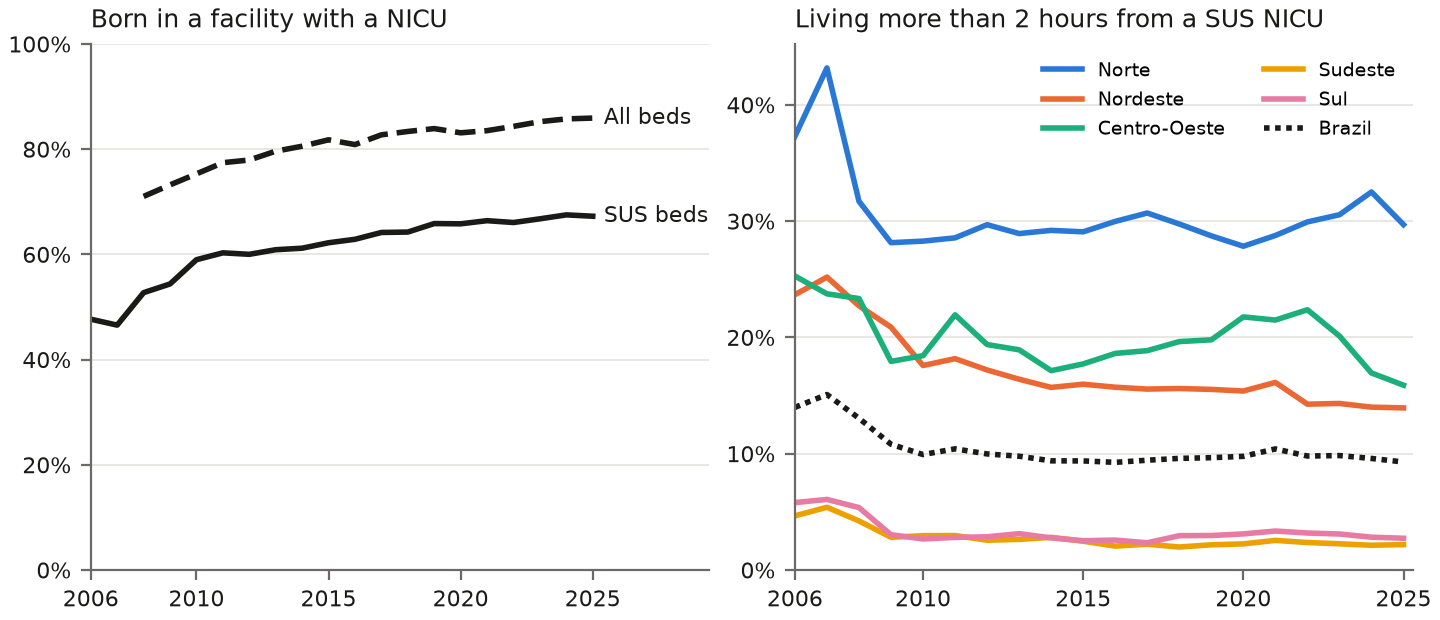
\includegraphics[width=\textwidth]{access.png}
\caption{Births of 500 to 1,499\,g, \firstYear--\lastYear. Left, share born in a
facility with a NICU, counting SUS beds and, from \allBedsFrom, every bed. Right,
share living more than two hours from a SUS NICU by region. 2007 is read in
November, \lastYear{} is preliminary.}
\label{fig:access}
\end{figure}

\subsection{Where the beds went}
SUS NICU beds grew by \bedsChange{} between \firstYear{} and \lastYear. Of these,
\bedsWherePresent{} were added in municipalities that already had a unit and
\bedsNewMunicipalities{} in the \munOpened{} municipalities that opened their
first one, while \munClosed{} municipalities lost all their SUS NICU beds
(\bedsLostClosed{} beds). Municipalities with a SUS NICU went from \munFirst{} to
\munLast.

Of the \munOpened{} municipalities that opened their first unit,
\munOpenedBeyond{} were more than two hours from any unit in \firstYear, with
\bedsOpenedBeyond{} beds in \lastYear. The others opened within reach of an
existing unit. Held at their \firstYear{} distribution, the \uncoveredFirst{}
births at risk that lived more than two hours away in \firstYear{} would number
\uncoveredLastMap{} with the units of \lastYear{} (\uncoveredLastMapShare). The
new units brought \broughtWithin{} of them within reach (\broughtWithinShare),
and \fellOut{} births of covered municipalities fell out of reach where units
closed.

The share beyond two hours changed by \changeTotal{} percentage points between
\firstYear{} and \lastYear. The new map of units accounts for \bedsEffect{}
points and the change in where births take place for \birthsEffect{} points.
Births at risk moved towards regions farther from units, the North holding
\norteRiskShareFirst{} of them in \firstYear{} and \norteRiskShareLast{} in
\lastYear, so part of what the new units gained was taken back by the geography
of births. Counting every bed from \allBedsFrom, the change is \allChangeTotal{}
points, \allBedsEffect{} from beds and \allBirthsEffect{} from births.

\subsection{Where to open the next units}
Over \pooledYears, \uncoveredPooled{} births at risk lived more than two hours
from a SUS NICU, about \uncoveredPerYear{} a year. Five new units would bring
\coverFive{} of them within two hours (\shareFive), ten \coverTen{} (\shareTen)
and twenty \coverTwenty{} (\shareTwenty). A unit in every one of the
\candidates{} candidates would cover \ceiling{} (\ceilingShare). The other
\beyondCeiling{} births live too far from any municipality large enough to hold a
unit, and new units alone will not reach them. Ten units cover \tenNinetyShare{}
of the uncovered births at 90 minutes, \tenOneEightyShare{} at three hours and
\tenLineShare{} under straight-line distances.

Table~\ref{tab:sites} lists the ten sites and figure~\ref{fig:map} places them.
\topSite{} comes first, with \topSitePerYear{} births at risk a year that live
beyond two hours today and would be within reach. The choices differ in how solid
they are. \solidSites{} are chosen in at least four of the five years taken alone
and under straight-line distances. \fragileSites{} are chosen in at most one year
alone, and the pooled answer rests on a few births that come and go. Only
\norteSites{} of the ten sites are in the North, which holds \norteFarShare{} of
the uncovered births of \pooledYears. Its municipalities are far apart and each
candidate reaches few births, so a model that maximises the number of births
covered favours the denser Northeast. The model counts births and does not weigh
equity between regions, and the gap of the North is not one that fixed units
within two hours can close.

\begin{table}[t]
\centering
\caption{The ten sites of the location model, births of \pooledYears{} against
the SUS units of \lastYear. Births reached are births at risk a year, living more
than two hours from any SUS NICU, that the site would bring within two hours. Years chosen counts the years, out of five, in which the model solved on
that year alone also chooses the site.}
\label{tab:sites}
\small
% Written by `nicu report` - do not edit by hand.
\begin{tabular}{llrcccc}
\toprule
 & & Births & Years & \multicolumn{2}{c}{Also chosen at} & Straight \\
\cmidrule(lr){5-6}
Municipality & State & reached a year & chosen & 90 min & 180 min & line \\
\midrule
Arcoverde & PE & 106 & 4 of 5 &  &  & $\bullet$ \\
Jacobina & BA & 74 & 5 of 5 & $\bullet$ &  & $\bullet$ \\
Rolim de Moura & RO & 66 & 1 of 5 & $\bullet$ &  &  \\
Antas & BA & 61 & 3 of 5 & $\bullet$ &  &  \\
Santo Antônio de Jesus & BA & 58 & 4 of 5 & $\bullet$ &  &  \\
Juruti & PA & 54 & 3 of 5 &  &  &  \\
Eunápolis & BA & 51 & 3 of 5 & $\bullet$ &  & $\bullet$ \\
Rio das Ostras & RJ & 45 & 2 of 5 & $\bullet$ &  & $\bullet$ \\
Barra do Corda & MA & 45 & 3 of 5 &  & $\bullet$ &  \\
Crateús & CE & 43 & 1 of 5 &  &  &  \\
\bottomrule
\end{tabular}

\end{table}

\section{Limits}
The transport network dates from 2016 and is applied to the whole period. Travel
times are those of scheduled public transport, slower than a car or an ambulance
and closer to what most families face. A municipality is reduced to its seat, so
distances inside a municipality count as zero, which flatters the large
municipalities of the North. SINASC records where a child was born, not where it
was treated, and transfers after birth would need hospital admission records.
Beds are those declared in the register, once a year, without their occupancy,
staffing or level of care. Weight leaves out preterm births of normal weight
that also need intensive care, so demand is a floor. Data for \lastYear{} are
preliminary. The location model assumes that a new unit serves every birth
within the travel time, whatever its size, and says nothing of cost. It maximises
the number of births covered and does not weigh equity between regions.

\section{Reproducibility}
The pipeline is a Python command line, \texttt{nicu}. \texttt{nicu ingest}
fetches the raw files and records each one in a manifest, \texttt{nicu build}
reduces them with DuckDB to counts by year, municipality and facility,
\texttt{nicu analyze} answers the three questions and \texttt{nicu report} writes
every number, table and figure of this note. Some sentences state a fact about
the data rather than a number, such as the North remaining the region farthest
from a unit, and \texttt{nicu report} checks each of them and stops if the data
no longer supports it. The counts and results are versioned, so the analysis and
this note can be rebuilt from a clone without downloading the raw files.
Continuous integration runs the tests, rebuilds the numbers of the note from the
versioned results, checks that they match the committed ones and compiles the
note. Design choices are recorded as decision records in the repository,
\texttt{github.com/paulianne-fontoura/nicu-access-brazil}, and the code is under
the MIT licence.

\begin{figure}[p]
\centering
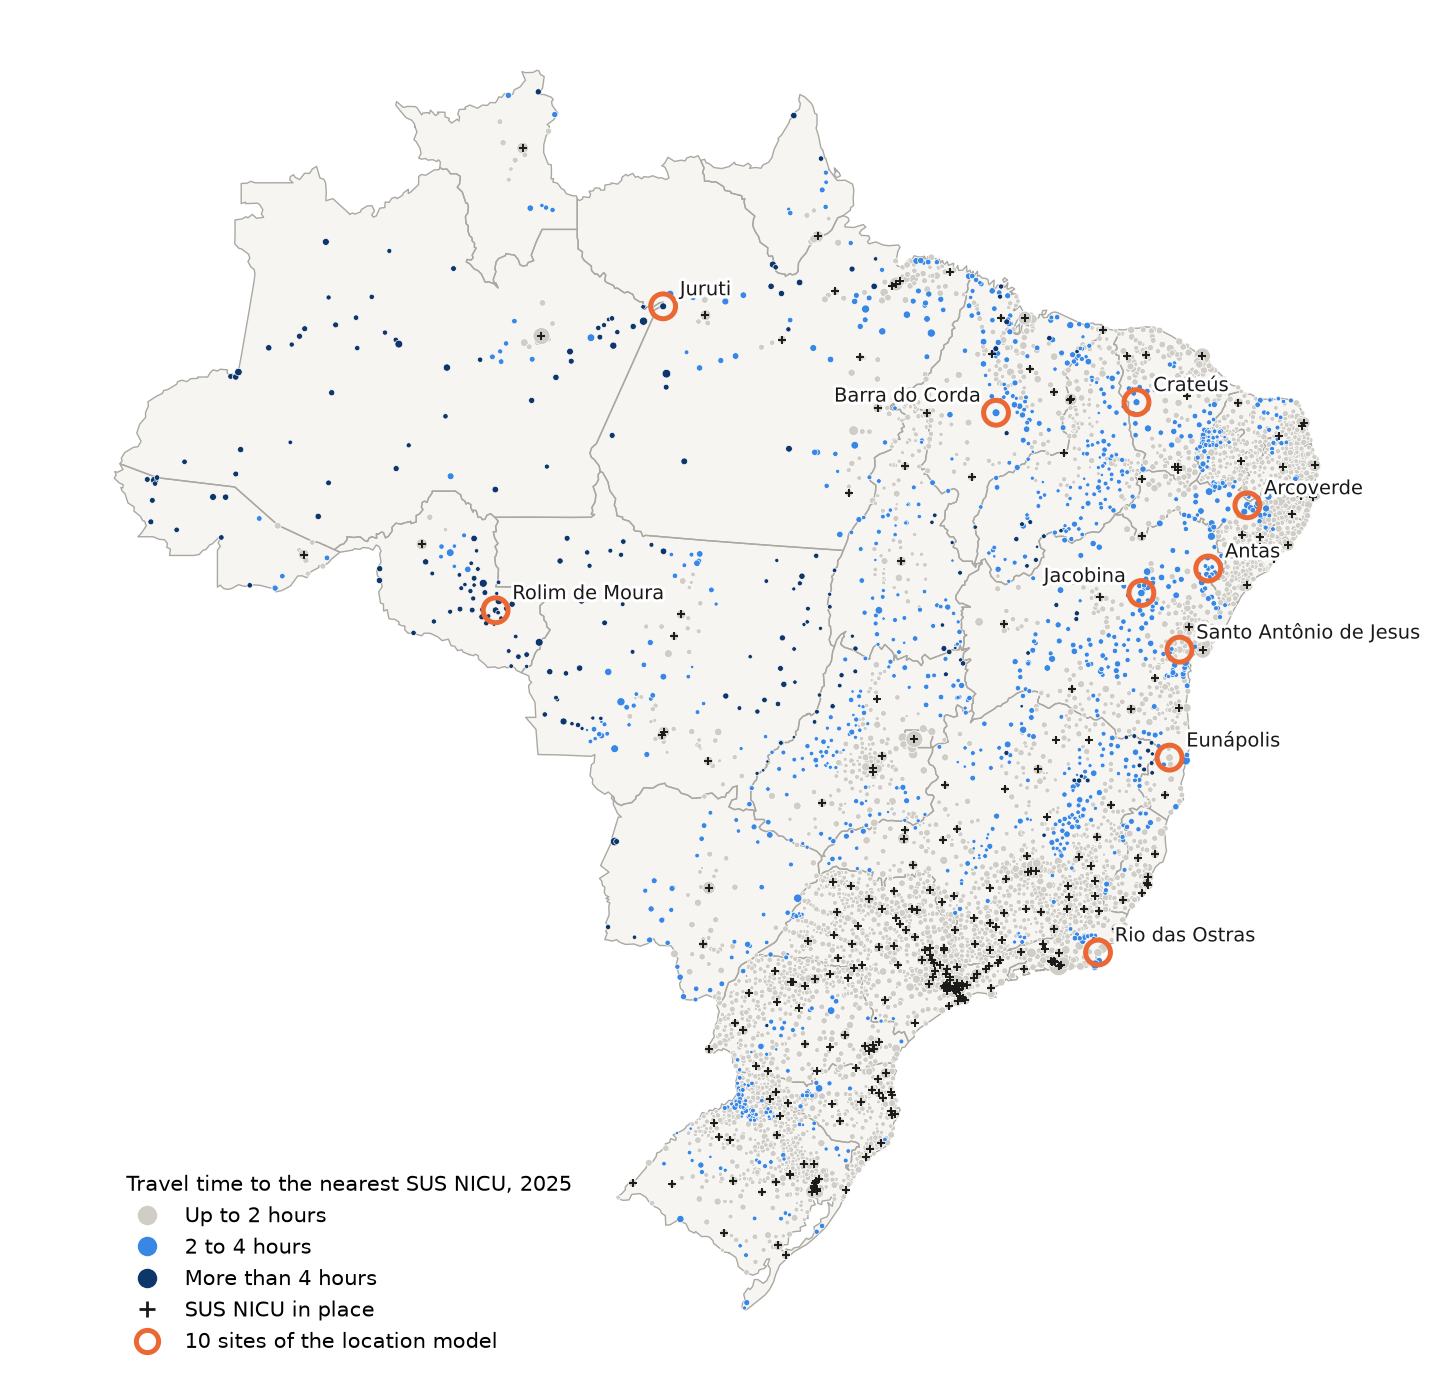
\includegraphics[width=\textwidth]{map.png}
\caption{Travel time from each municipality to the nearest SUS NICU in
\lastYear{} on the bus and boat network. Dot size follows the births of 500 to
1,499\,g of \pooledYears{} by municipality of residence. Crosses mark the
municipalities with a SUS NICU, circles the ten sites of the location model at
two hours.}
\label{fig:map}
\end{figure}

\end{document}
